\section{Algorithm}
\label{sec:parmaparmaalgo}
In this section we describe and analyze PARMA, our algorithm for extracting
$\varepsilon$-close approximations of $\FI(\Ds,\Itm,\theta)$,
$\TOPK(\Ds,\Itm,\theta)$, and $\AR(\Ds,\Itm,\theta,\gamma)$ from samples of a dataset
$\Ds$ with probability at least $1-\delta$. In this section we present the
variant for the absolute case and $\FI(\Ds,\Itm,\theta)$. The variants for the
relative cases and for $\TOPK(\Ds,\Itm,\theta)$ and
$\AR(\Ds,\Itm,\theta,\gamma)$ can be easily derived from the one
we present here. We outline them in Section~\ref{sec:parmaeapproxtopk}. 

\subsection{Design}\label{subsec:parmadesign}
We now present the algorithmic design framework on which we developed PARMA and
some design decisions we made for speeding up the computation. 

\paragraph*{Model}When developing solutions for any computational problem,
the algorithm designer must always be aware of the trade-off between the available
computational resources and the performance (broadly defined) of the algorithm.
In the parallel computation setting, the resources are usually modeled through
the parameters $p$ and $m$, representing respectively the number of available
processors that can run in parallel and the amount of local memory available to
a single processor. In our case we will express $m$ in terms of the number of
transactions that can be stored in the main memory of a single machine.
When dealing with algorithms that use random samples of the input, the
performances of the algorithm are usually measured through the parameters
$\varepsilon$ and $\delta$. The former represents the desired accuracy of the
results, i.e., the maximum tolerable error (defined according to some distance
measure) in the solution computed by the algorithm using the random sample
when compared to an exact solution of the computational problem. The parameter
$\delta$ represents the maximum acceptable probability that the previously
defined error in the solution computed by the algorithm is greater than
$\varepsilon$. The measure we will use to evaluate the performances of PARMA in
our analysis is based on the concept of absolute $\varepsilon$-close
approximation introduced in Definition~\ref{def:parmaeapproxfi}.

\paragraph*{Trade-offs} We are presented with a trade-off between the parameters
$\varepsilon$, $\delta$, $p$, and $m$. To obtain a $\varepsilon$-approximation
with probability at least $1-\delta$, one must have a certain amount of computational resources,
expressed by $p$ and $m$. On the other hand, given $p$ and $m$, it is possible
to obtain absolute $\varepsilon$-close approximations with probability at least
$1-\delta$ only for values of $\varepsilon$ and $\delta$ larger than some
limits. By fixing any three of the parameters, it is possible to find the
best value for the fourth by solving an optimization problem. From
Lemma~\ref{lem:absapproxfi} we know that there is a trade-off between
$\varepsilon$, $\delta$, and the size $w$ of a random sample from which it is
possible to extract a $(\varepsilon,\varepsilon/2)$-approximation to
$\FI(\Ds,\Itm,\theta)$ with probability at least $1-\delta$. If $w\le m$, then
we can store the sample in a single machine and compute the absolute
$\varepsilon$-close approximation there using Lemma~\ref{lem:absapproxfi}. For some
combinations of values for $\varepsilon$ and $\delta$, though, we may have that
$w>m$, i.e. the sample would be too large to fit into the main memory of a single
processor, defeating one of the goals of using random sampling, that is to store
the set of transactions to be mined in main memory in order to avoid expensive disk
accesses. To address the issue of a single sample not fitting in memory, PARMA
works on multiple samples, say $N$ with $N\le p$, each of size $w\le m$ so that
{\bf 1)} each sample fits in the main memory of a single processor and {\bf 2)}
for each sample, it is possible to extract an absolute
$(\varepsilon,\varepsilon/2)$-close approximation of $\FI(\Ds,\Itm,\theta)$ from it
with probability at least $1-\phi$, for some $\phi>\delta$. In the first stage,
the samples are created and mined in parallel and the so-obtained collections of
Frequent Itemset are then aggregated in a second stage to compute the final output. This
approach is a perfect match for the MapReduce framework, given the limited
number of synchronization and
communication steps that are needed. Each
stage is performed in a single MapReduce round. The computational and data
workflow of PARMA is presented in Figure~\ref{fig:parmaoverview}, which we
describe in detail in the following paragraphs.

\begin{figure}[htb]
\centering
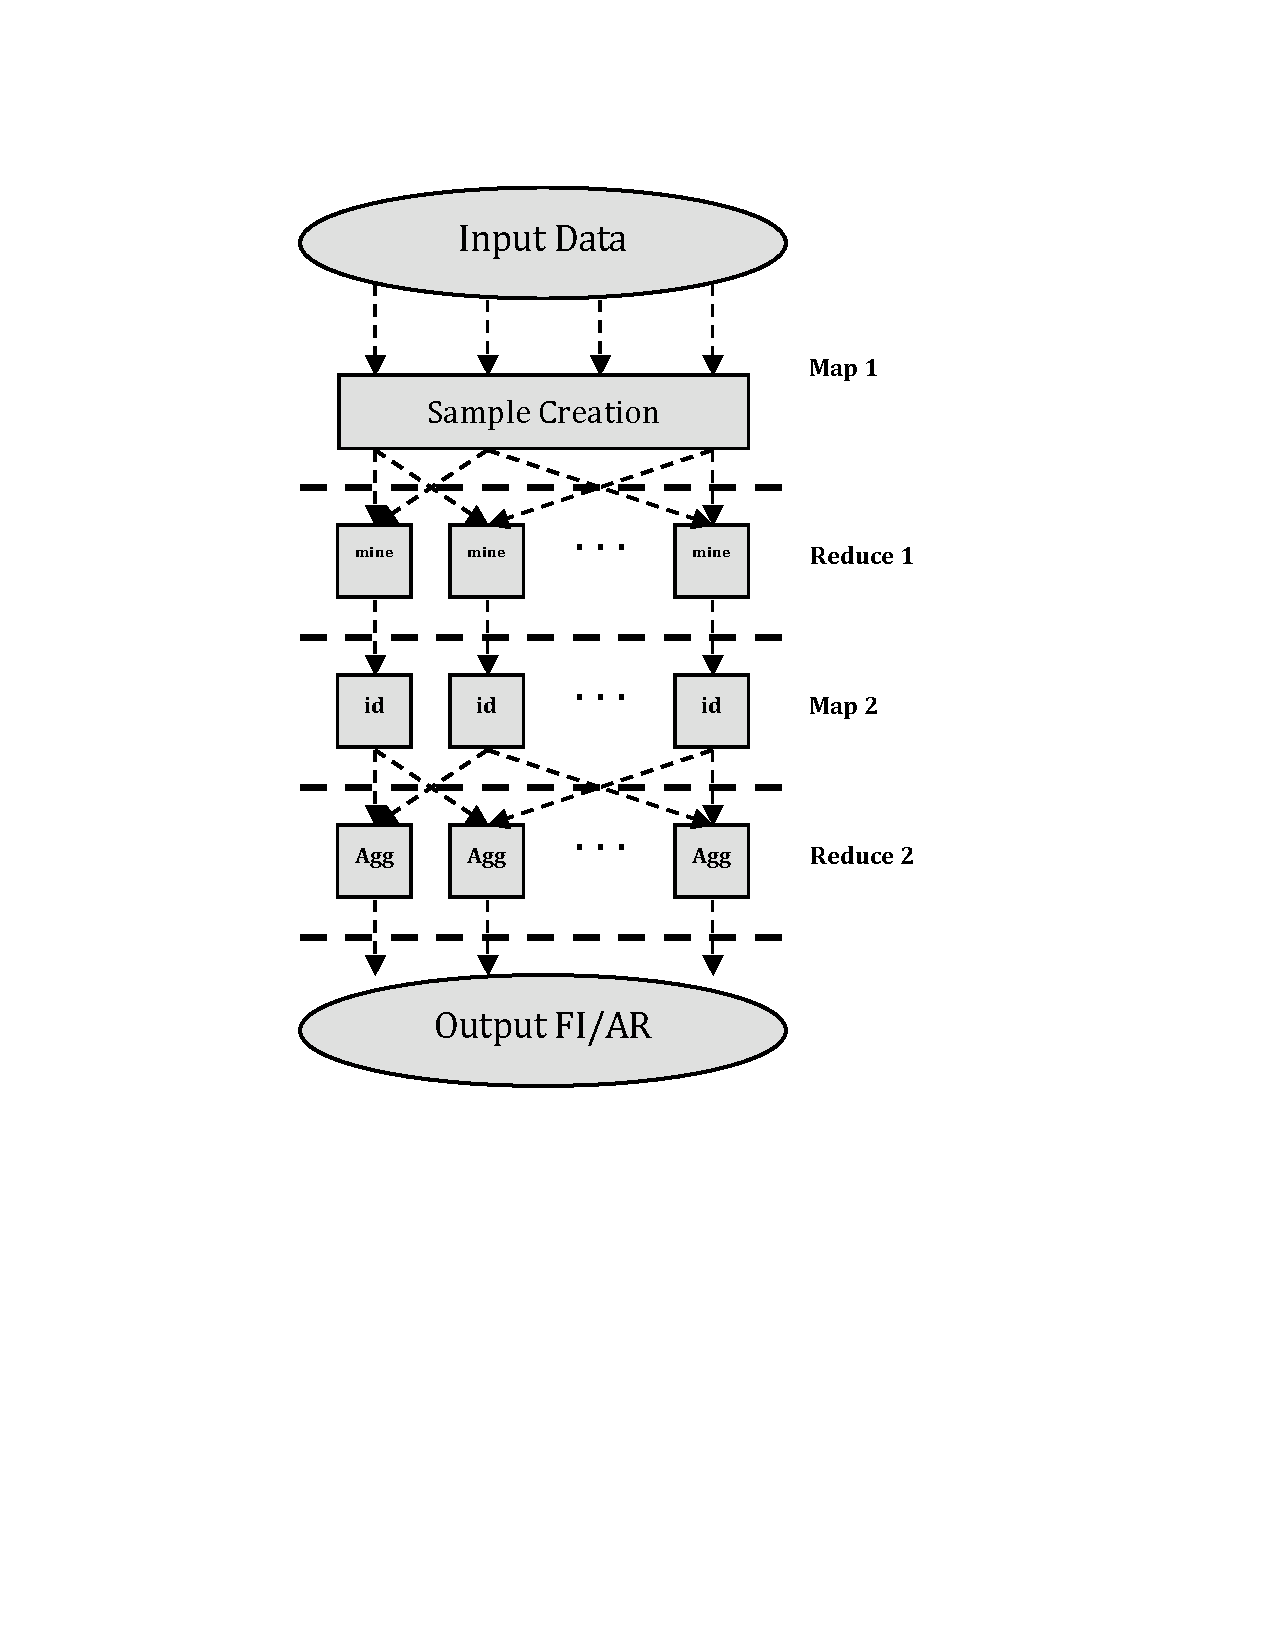
\includegraphics[width=0.4\textwidth]{parma/overview.pdf}
\caption{A system overview of PARMA. Ellipses represent data, squares represent
computations on that data and arrows show the movement of data through the
system.}
\label{fig:parmaoverview}
\end{figure}

  \begin{comment}
  The diagram is broken into 4 main computations which correspond to the
  Map and Reduce phases of the two MapReduce rounds in the algorithm. In
  the Map of Stage 1, a sample is created. In the Reduce of Stage 1, a
  mining algorithm is run on the subset of the sample created in the Map
  phase. This mining algorithm can be either frequent itemset mining or
  association rule mining, and as such is generically labeled mine. In
  the Map phase of Stage 2, the local frequent itemsets are sent to an
  identity mapper, and finally Aggregated in the Stage 2 Reduce to get a
  global set of frequent itemsets or assocation rules, depending on the
  mining algorithm used.
\end{comment}


\paragraph*{Computing $N$ and $w$} From the above discussion it should be clear
that, once $p$, $m$, $\varepsilon$ and $\delta$ have been fixed, there is a
trade-off between $w$ and $N$. In the MapReduce setting, often the most expensive
operation is the movement of data between the mappers and the reducers in the
shuffle phase. In PARMA, the amount of data to be shuffled corresponds to the
sum of the sizes of the samples, i.e., $Nw$, and to the amount of
communication needed in the aggregation stage. This second quantity is dependent
on the number of frequent itemsets in the dataset, and therefore PARMA has no
control over it. PARMA tries to minimize the first quantity when computing $N$ and
$w$ in order to achieve the maximum speed. It is still possible to minimize for
other quantities (e.g. $\varepsilon$ or $\delta$ if they have not been fixed),
but we believe the most effective and natural in the MapReduce setting is the
minimization of the communication.  This intuition was verified in our
experimental evaluation, where communication proved to be the dominant cost. We
can formulate the problem of minimizing $Nw$ as the following Mixed Integer Non
Linear Programming (MINLP) problem:
\begin{itemize}
  \item {\bf Variables:} non-negative integer $N$, real $\phi\in(0,1)$,
  \item {\bf Objective:} minimize $2N/\varepsilon^2 (d+\log(1/\phi))$.
  \item {\bf Constraints:}
    \begin{align}
      &N \le p \label{eq:parmaconstr1}\\
      &\phi \ge e^{-m\varepsilon^2/2 + d} \label{eq:parmaconstr2}\\
      &N(1-\phi)-\sqrt{N(1-\phi)2\log(1/\delta)} \ge N/2 + 1 \label{eq:parmaconstr3}
    \end{align}
\end{itemize}
Note that, because of our requirement {\bf 2)} on $w$, the sample size $w$ is directly
determined by $\phi$ through Lemma~\ref{lem:absapproxfi}, so the trade-off is
really between $N$ and $\phi$, while $w$ does not appear in the above problem.
Since $\phi$ is a probability we restrict its
domain to the interval $(0,1)$, but it must also be such that the single sample size
$w$ is at most $m$, as required by {\bf 1)} and expressed by
Constraint~\eqref{eq:parmaconstr2}. The limit to the number of samples $N$ is expressed by
Constraint~\eqref{eq:parmaconstr1}. The last constraint~\eqref{eq:parmaconstr3} is a bit
more technical and the need for it will be evident in the analysis of the
algorithm. Intuitively, it expresses the fact that an itemset must appear in a
sufficiently high fraction (at least 1/2, possibly more) of the collections obtained from the samples in the
first stage in order to be included in the output collection. Due to the integrality constraint on
$N$, this optimization problem is not convex, although when the constraint it is
dropped the feasibility region is convex, and the objective function is convex.
It is then relatively easy and fast to find an integer optimal solution to the
problem using a global MINLP solver like BARON~\citep{baron}. 


\subsection{Description}
In the following paragraphs we give a detailed description of PARMA. The reader
is also referred to Figure~\ref{fig:parmaoverview} for a schematic representation of
PARMA's data/computational workflow.

\paragraph*{Stage 1: Sampling and Local Mining} Once $\phi$, $w$
and $N$ have been computed, PARMA enters the first MapReduce round to create
the $N$ samples (phase Map 1 in Figure~\ref{fig:parmaoverview}) and mine them (Reduce 1).
We see the input of the algorithm as a sequence
\[
(1,\tau_1),(2,\tau_2),\cdots,(|\Ds|,\tau_{|\Ds|}),\]
where the $\tau_i$ are transactions in $\Ds$.
In the Map phase, the input of the {\bf map} function is a pair $(tid, \tau)$, where
$tid$ is a natural from $1$ to $|\Ds|$ and $\tau$ is a transaction in $\Ds$. The
map function produces in output a pair $(i,(\ell^{(i)}_\tau,\tau))$ for each
sample $\Sam_i$ containing $\tau$. The value $\ell^{(i)}_\tau$ denotes the
number of times $\tau$ appears in $\Sam_i$, $1\le i \le N$. We use random sampling
with replacement and ensure that all samples have size $w$, i.e.,
$\sum_{\tau\in\Ds}\ell^{(i)}_\tau=w$, $\forall i$. This is done by computing
(serially) how many transactions each mapper must send to each sample. In the
Reduce phase, there are $N$ reducers, with associated key $i$, $1\le i \le N$.
The input to reducer $i$ is $(i,\Sam_i)$, $1\le i\le N$. Reducer $i$ mines the
set $\Sam_i$ of transactions it receives using an exact sequential mining
algorithm like Apriori or FP-Growth and a lowered minimum frequency threshold
$\theta'=\theta-\varepsilon/2$ to obtain
$\mathcal{C}_i=\FI(\Sam_i,\Itm,\theta')$. For each itemset $A\in\mathcal{C}_i$
the Reduce function outputs a pair $(A,
(f_{\Sam_i}(A),[f_{\Sam_i}(A)-\varepsilon/2,f_{\Sam_i}(A)+\varepsilon/2])$.

\paragraph*{Stage 2: Aggregation} In the second round of MapReduce, PARMA
aggregates the result from the first stage to obtain an absolute
$\varepsilon$-close approximation to $\FI(\Ds,\Itm,\theta)$ with probability at least
$1-\delta$. The Map phase (Map 2 in Figure~\ref{fig:parmaoverview}) is just the identity
function, so for each pair 
\[(A,
(f_{\Sam_i}(A),[f_{\Sam_i}(A)-\varepsilon/2,f_{\Sam_i}(A)+\varepsilon/2])\]
in the input the same pair is produced in the output. In the Reduce phase (Reduce 2) there
is a reducer for each itemset $A$ that appears in at least one of the
collections $\mathcal{C}_j$ (i.e., $\forall A$ such that there is a
$\mathcal{C}_j$ containing a pair related to $A$). The reducer receives as input
the itemset $A$ and the set $\mathcal{F}_A$ of pairs
\[
(f_{\Sam_i}(A),[f_{\Sam_i}(A)-\varepsilon/2,f_{\Sam_i}(A)+\varepsilon/2])\]
for the samples $\Sam_i$ such that $A\in\mathcal{C}_i$.
Now let
\begin{equation}\label{eq:parmaRdef}
R = N(1-\phi)-\sqrt{N(1-\phi)2\log(1/\delta)}.
\end{equation}
The itemset $A$ is declared
\emph{globally frequent} and will be present in the output if and only if
$|\mathcal{F}_A| \ge R$. If this is the case, PARMA computes, during the Reduce
phase of the second MapReduce round, the estimation $\tilde{f}(A)$ for the
frequency $f_\Ds(A)$ of the itemset $A$ in $\Ds$ and the confidence interval
$\mathcal{K}_A$. The computation for $\tilde{f}(A)$ proceeds as follows. Let
$[a_A,b_A]$ be the \emph{shortest} interval such that
there are at least $N-R+1$ elements from $\mathcal{F}_A$ that belong to this
interval. The estimation $\tilde{f}(A)$ for the frequency $f_\Ds(A)$ of the
itemset $A$ is the central point of this interval:
\[ \tilde{f}(A)=a_A+\frac{b_A-a_A}{2}\]
The confidence interval $\mathcal{K}_A$ is defined as
\[ \mathcal{K}_A=\left[a_A-\frac{\varepsilon}{2},b_A+\frac{\varepsilon}{2}\right].\]
The output of the reducer assigned to the itemset $A$ is \[(A,(\tilde{f}(A),\mathcal{K}_A)).\]
The output of PARMA is the union of the outputs from all reducers.

\subsection{Analysis}
We have the following result:
\begin{lemma}\label{lem:multiepsapprox}
 The output of the PARMA is an absolute $\varepsilon$-close approximation of
 $\FI(\Ds,\Itm,\theta)$ with probability at least $1-\delta$.
\end{lemma}

\begin{proof}
  For each sample $\Sam_i$, $1\le i\le N$ we define a random variable $X_i$ that
  takes the value $1$ if $\mathcal{C}_i=\FI(\Sam_i,\Itm,\theta')$ is an absolute
  $(\varepsilon,\varepsilon/2)$-close approximation of $\FI(\Ds,\Itm,\theta)$, $X_i=0$
  otherwise. Given our choices of $w$ and $\theta'$, we can apply
  Lemma~\ref{lem:absapproxfi} and have that $\Pr(X_i=1)\ge 1-\phi$. Let
  $Y=\sum_{r=1}^N X_r$ and let $Z$ be a random variable with binomial
  distribution with parameters $N$ and $1-\phi$. For any constant $Q<N(1-\phi)$ we have
  \[
  \Pr(Y\le Q)\le\Pr(Z\le Q)\le e^{-N(1-\phi)(1-\frac{Q}{N(1-\phi)})^2/2},
  \]
  where the last inequality follows from an application of the Chernoff
  bound~\cite[Chap.~4]{MitzenmacherU05}.
  We then have, for our choice of $\phi$ and $N$ and for $Q=R$
  (defined in Eq.~\eqref{eq:parmaRdef}), that with probability at least $1-\delta$,
  at least $R$ of the collections $\mathcal{C}_i$ are absolute
  $(\varepsilon,\varepsilon/2)$-close approximations of $\FI(\Ds,\Itm,\theta)$. Denote
  this event as $\mathcal{G}$. For the rest of the proof we will assume that
  $\mathcal{G}$ indeed occurs.

  Then $\forall A\in\FI(\Ds,\Itm,\theta)$, $A$ belongs to at least $R$ of the
  collections $\mathcal{C}_i$, therefore a triplet
  $(A,\tilde{f}(A),\mathcal{K}_A)$ will be in the output of the algorithm. This
  means that Property 1 from Def.~\ref{def:parmaeapproxfi} holds. 

  Consider now any itemset $B$ such that $f_\Ds(B)<\theta-\varepsilon$. By
  definition of absolute $(\varepsilon,\varepsilon/2)$-close approximation we have that $B$ can
  only appear in the collections $\mathcal{C}_i$ that are not absolute
  $(\varepsilon,\varepsilon/2)$-close approximations. Given
  that $\mathcal{G}$ occurs, then there are at most  $N-R$ such collections. But
  from Constraint~\eqref{eq:parmaconstr3} and the definition of $R$
  in~\eqref{eq:parmaRdef}, we have that $N-R< R$, and therefore $B$ will not be
  present in the output of PARMA, i.e.~Property 2 from Def.~\ref{def:parmaeapproxfi} holds.

  Let now $C$ be any itemset in the output, and consider the interval
  $S_C=[a_C,b_C]$ as computed by PARMA. $S_C$ contains at least $N-R+1$ of
  the $f_{\Sam_i}(C)$, otherwise $C$ would not be in the output. By our
  assumption on the event $\mathcal{G}$, we have
  that at least $R$ of the $f_{\Sam_i}(C)$'s are such that
  $|f_{\Sam_i}(C)-f_\Ds(C)|\le\varepsilon/2$. Then there is an index $j$ such
  that $|f_{\Sam_j}(C)-f_\Ds(C)|\le\varepsilon/2$ and such that
  $f_{\Sam_j}(C)\in S_C$.
  Given also that $f_{\Sam_j}(C)\ge a_C$, then $f_\Ds(C)\ge
  a_C-\varepsilon/2$, and analogously, given that $f_{\Sam_j}(C)\le b_C$, then
  $f_\Ds(C)\le b_C+\varepsilon/2$. This means that
  \begin{equation}\label{eq:parmasingleepsapproxinterval}
    f_\Ds(C)\in
    \left[a_C-\frac{\varepsilon}{2},
    b_C+\frac{\varepsilon}{2}\right]=\mathcal{K}_C,
  \end{equation}
  which, together with the fact that $\tilde{f}_C\in\mathcal{K}_C$ by
  construction, proves Property 3.b from Def.~\ref{def:parmaeapproxfi}.
  We now give a bound to $|S_C|=b_C-a_C$. From our
  assumption on the event $\mathcal{G}$, there are (at least) $R$ values
  $f_{\Sam_i}(C)$ such that $|f_{\Sam_i}(C)-f_\Ds(C)|\le\varepsilon/2$, then the
  interval $[f_\Ds(C)-\varepsilon/2,f_\Ds(C)+\varepsilon/2]$ contains (at least)
  $R$ values $f_{\Sam_i}(C)$. Its length $\varepsilon$ is an upper bound to
  $|S_C|$. Then the length of the interval
  $\mathcal{K}_C=[a_C-\varepsilon/2,b_C+\varepsilon/2]$ is at most
  $2\varepsilon$, as requested by Property 3.c from
  Def.~\ref{def:parmaeapproxfi}. From this, from ~\eqref{eq:parmasingleepsapproxinterval}, and
  from the fact that $\tilde{f}(C)$ is the center of this interval we have
  $|\tilde{f}(C)-f_\Ds(C)|\le\varepsilon$, i.e., Property 3.a from
  Def.~\ref{def:parmaeapproxfi} holds.
\end{proof}

\subsection{Top-K Frequent Itemsets and Association Rules}\label{sec:parmaeapproxtopk}
The above algorithm can be easily adapted to computing, with probability at
least $1-\delta$, absolute and relative $\varepsilon$-close approximations to $\TOPK(\Ds,\Itm,K)$ and to
$\AR(\Ds,\Itm,\theta,\gamma)$. The main difference is in the formula to compute
the sample size $w$ (Lemma~\ref{lem:absapproxfi}), and in the process
to extract the local collections from the samples. The case of top-$K$ is
presented in Lemma~\ref{lem:absapproxtopk}, while for the association rule case
we can use Lemma~\ref{lem:absapproxar}. These are minimal changes to the version
of PARMA presented here, and the modified algorithms guarantee the same levels
of accuracy and confidence.

%main difference is in the formula to compute sample size $w$
%(Eq.~\eqref{eq:parmasinglesamplesize}, which in this case is set to $w=8(d+\log
%1/\phi)/varepsilon^2$, and in the work done by the reducers in the
%first phase: using the algorithm presented in~\cite[Lemma 3]{RiondatoU12}, each
%reducer $r$ computes, with probability at least $1-\phi$, a collection
%$\mathcal{C}_r$ such that if we see $\TOPK(\Ds,\Itm,K)$ as
%$\FI(\Ds,\Itm,f^{(K)}_\Ds)$, $\mathcal{C}_r$ is a
%$(\varepsilon,\varepsilon/2)$-approximation to $\FI(\Ds,\Itm,f^{(K)}_\Ds)$. The
%collections $\mathcal{C}_i$'s are then aggregated in the second MapReduce round
%in the same way as for the case of FI's  described in the previous section. This
%result is formulated in the following Lemma, whose proof will be included in the
%full version of the paper. 
%\begin{lemma}
%   The output of the algorithm is an $\varepsilon$-approximation of
%   $\TOPK(\Ds,\Itm,K)$ with probability at least $1-\delta$.
%\end{lemma}
%
%\subsection{Association Rules}\label{sec:parmaeapproxar}
%The above algorithm can be easily adapted to computing, with probability at
%least $1-\delta$, an $\varepsilon$-approximation to
%$\AR(\Ds,\Itm,\theta,\gamma)$. The main differences are again in how to compute
%the sample size $w$ (see Lemma~\ref{lem:absapproxar}) and in the work done by the
%reducers in the first phase. Using the algorithm presented in~\cite[Lemma
%6]{RiondatoU12}, each reducer $r$ computes a collection $\mathcal{C}_r$ such
%that $\mathcal{C}_r$ is a $(\varepsilon,\varepsilon/2)$-approximation to
%$\AR(\Ds,\Itm,\theta,\gamma)$  with probability at least
%$1-\phi$, The collections $\mathcal{C}_r$ are then aggregated in the second
%MapReduce phase as described in the previous section, with the only addition of
%computing an estimate $\tilde{g}(W)$ for the confidence $g_\Ds(W)$ of each
%association rule $W$ in the output, and an interval $\mathcal{J}(W)$. This can be
%done exactly in the same way as computing the estimate $\tilde{f}(W)$ for the
%frequency $f_\Ds(W)$ and the corresponding interval $\mathcal{K}(W)$. The
%properties of the output are formulated in the following Lemma, whose proof will
%be included in the full version of the paper.
%\begin{lemma}
%   The output of the algorithm is an $\varepsilon$-approximation of
%   $\AR(\Ds,\Itm,\theta,\gamma)$ with probability at least $1-\delta$.
%\end{lemma}
%
